\chapter{Evaluation}\label{ch:evaluation}
\color{blue}

In our tool, usability and user experience are very important. Therefore, we did two user studies. The first was to test the functionality of the GuideaMaps (as map creator and as end-user), while the second tested the use case about Plateforme DD.\\

This chapter is divided in two sections. The first describes the user study of GuideaMaps together with its results. In the second section, the same is done for the user study of Plateforme DD.





\section{GuideaMaps}
In this section, we describe the evaluation of the default implementation of the tool. With ``default'' we mean that no implementation is plugged in into the library but the standard visualization is used as described in \autoref{sec:default-implementation}.

\subsection{Setup}
The evaluation was split in two parts, each testing one of the two modes. In the first part, we tested the map creator mode. For this mode, we asked people with a background in Computer Science and/or visualization techniques to participate. As we expect end-users can be almost everyone, this was not a requirement to participate in the part testing the functionality of the end-user.\\

All participants answered the questions at home without additional explanation than the text provided at the beginning of the questionnaire.

\subsection{Tasks \& Questions}
For each mode, a different questionnaire was created (\autoref{appendix:gm-evaluation-map-creator} and \autoref{appendix:gm-evaluation-end-user}). They both start with a brief explanation about the tool, because nobody knew it or used it before. Before the actual questions, we ask the participant to enter his age and whether he has a background in Computer Science and/or visualization techniques or not.\\

This is followed by the questions concerning the functionality of the tool. The goal was to let the participants experience the actions a real map creator or end-user can perform. After each action, we ask to indicate how intuitive it was for them to get to the expected result. This can be very useful to know, e.g. when the majority indicates a certain action was not intuitive at all, we know something should be changed in the design of the tool. When all questions with tasks are answered, the participant should upload a screenshot of his screen, so that we can check whether everything went as intended.\\

Further, we wanted to test the usability of the tool. Therefore, we added a SUS usability questionnaire\footnote{\url{https://www.usability.gov/how-to-and-tools/methods/system-usability-scale.html}}.\\

The questionnaire was concluded with some open questions where the participant could provide his opinion. We asked to tell us what was good about the visualization and where they think we could have done better.

\subsection{Results}
We expect that participants taking the role of map creator will experience more tasks as intuitive than participants taking the role of end-user.




\section{Plateforme DD}
The evaluation of the use case about Plateforme DD is different in comparison to the one about GuideaMaps. A first difference is that our audience is different: for GuideaMaps we chose for participants with a background in Computer Science to take the role as map creator. The participants taking the role of end-user were also more than 20 years old. Now, for Plateforme DD, our audience is between ten and fifteen years old. This is because the content on the website\footnote{\url{https://sciences.brussels/dd/}} was created by children of similar ages \textcolor{red}{(TODO: check this)}. However, the participants of the user study never worked with the website before.

\subsection{Setup}
The children were divided in two groups: one group solved the questionnaire using the website, while the other group solved the same questionnaire using the application. There was one tablet per two children on which the website or the application was running (depending on the group they were in). It was important they did not work with both systems because then there was the possibility a learning effect of having used one system before the other could influence the results. 

\subsection{Tasks \& Questions}
The user study consisted of different tasks and questions the children had to solve. Before they started with the actual tasks and questions, we gave them five minutes to explore the website or the application so that they could get used to it a bit. We mentioned that it was important to understand the structure as much as possible because some questions would follow after this introduction period.\\

After five to ten minutes, we distributed the papers with the tasks and the questions. With other words, all children (of both groups) received part 1 of the questionnaire (see \autoref{appendix:pdd-questionnaire}). The first six questions of part 1 were about the understanding of the structure of the content. Then, four more questions were added to test the searching and finding of information in both systems. The participants using the application also had to answer four more questions about ``insight'' in the way the information is structured and linked. Participants using the website did not have to answer these questions because these are specific for the application.\\

After twenty minutes, all questionnaires of part 1 were collected, even if the participant did not finish all questions yet. Together with the pages, the tablets were collected as well because there are no questions left where the participants really needed the application or the website anymore. After collecting everything, part two of the questionnaire was distributed to all participants. In this part, the questions were not about the content or the structure of the information, but about usability and user experience. Hence, we wanted to know the opinion of the participants about the system they used so that we could compare which of the two systems they liked the most. The questions about usability and user experience can be found in \autoref{appendix:pdd-questionnaire} and \autoref{appendix:ueq-questionnaire}, respectively. The usability questions are based on the SUS questionnaire previously mentioned. Note that it is different than the SUS questionnaire for the evaluation of GuideaMaps. We adapted the questions a bit because not all questions were useful for our purpose.



\subsection{Results}
In general, we predict that participants using the application are better in answering most of the questions of part 1 correctly than the participants using the website. Certainly because they only have 20 minutes to answer all questions. We expect that not all participants using the website will be able to answer all questions in this amount of time. Even though we know it is possible that some participants using the application will not be able to finish the questionnaire either, we predict participants using the application will be able to answer more of the questions than participants using the website.

\subsubsection{Structure Comprehension}

\begin{figure}[H]
	\centering
	\frame{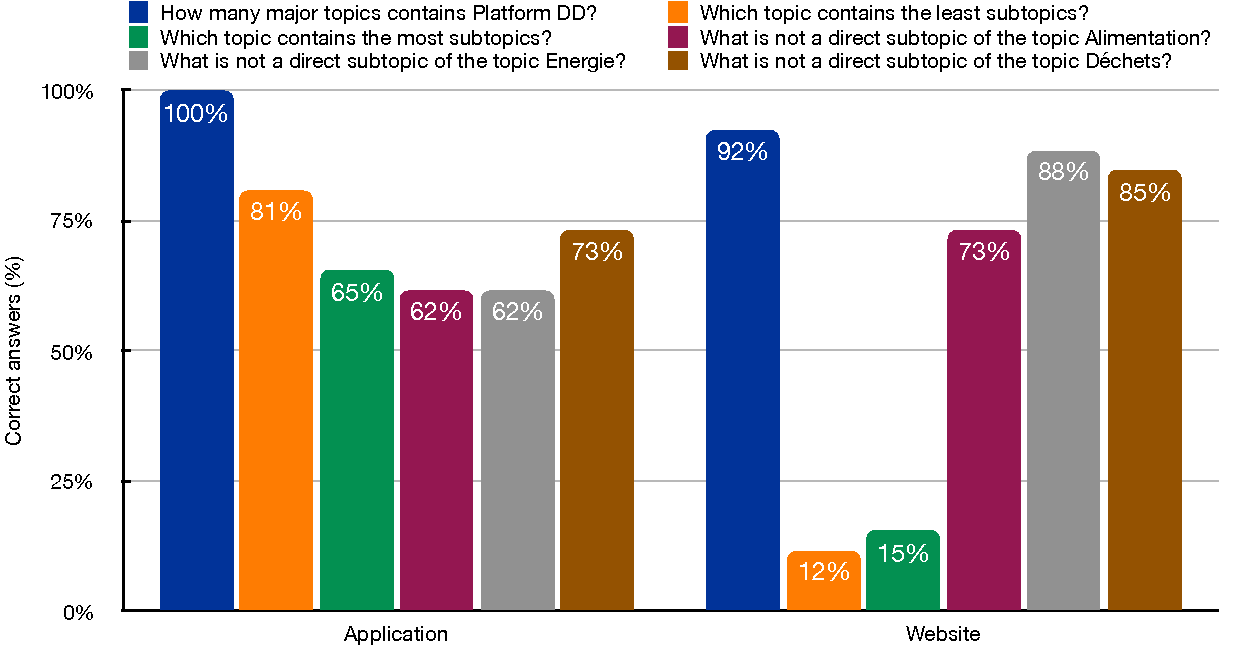
\includegraphics[width=\linewidth]{evaluation/part1-first6.pdf}}
	\caption{Results of the first 6 questions of part 1.}
	\label{fig:evaluation-pdd-first6}
\end{figure}

\autoref{fig:evaluation-pdd-first6} shows the results of the first six questions of the questionnaire. We can see that almost every participant correctly found that the content is divided over three major topics. But more important is that participants using the application were significantly better in finding which topic contains the most and which the least number of subtopics. We expected this because in the application, the tree structure is more clear. As a consequence, these users have a better overview than the participants using the website. To the questions about which is not a direct subtopic of a certain topic, the participants using the website gave a correct answer more frequently. This is probably because these users cannot see indirect subtopics of the topics in the questions. Participants using the application possibly made some indirect subtopics visible by clicking on the plus-button and were then a bit disturbed.

\subsubsection{Search \& Find}
After the first six questions, in which they discovered the structure of the content, we asked them to search and find information in the tool they were using. The results can be found in \autoref{fig:evaluation-pdd-search-find}. In general, we see that participants using the application are better in retrieving the information from the tool than the ones using the website.

\begin{figure}[H]
	\centering
	\frame{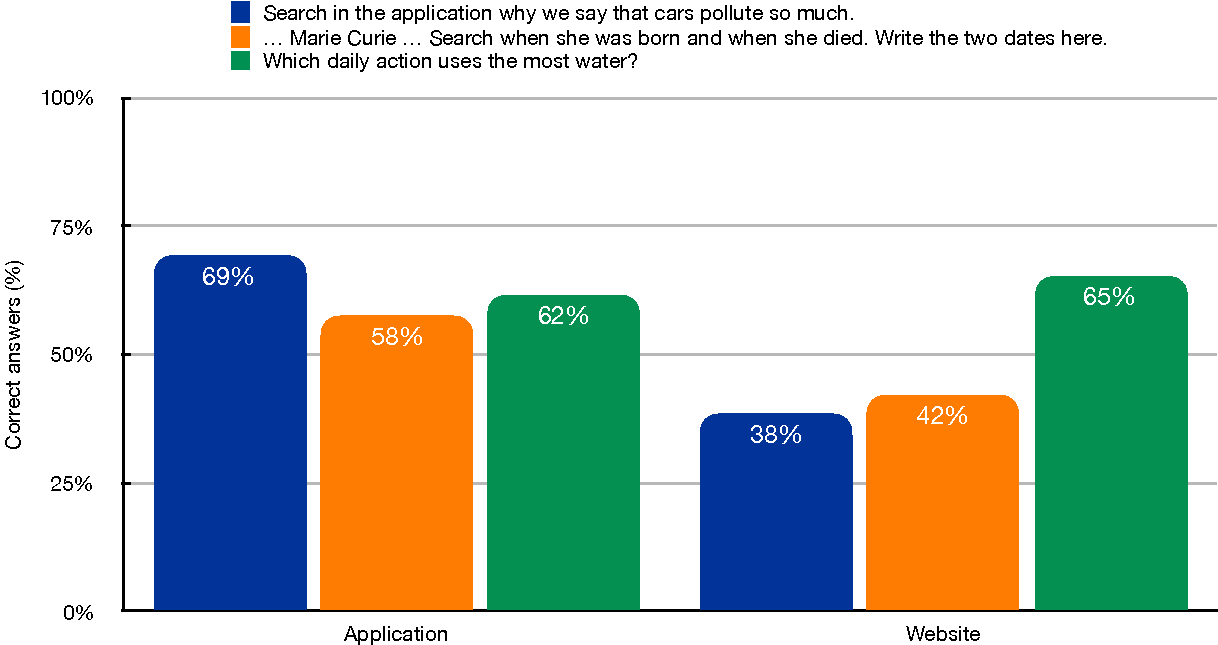
\includegraphics[width=\linewidth]{evaluation/part1-search-find.pdf}}
	\caption{Results of search \& find questions.}
	\label{fig:evaluation-pdd-search-find}
\end{figure}

We also asked them to write the titles as possible of topics which are still ``under construction''. This was not very successful because more than half of the participants could not find such a topic. The average number of topics found per participant is 0.42 in the case of the application and 0.81 in case of the website. This is probably because going through the topics on the website is quite fast, i.e. you just click on other topics until you find one that is under construction, while in the application you have to open and close the nodes one by one which takes more time.

\subsubsection{Insight}
The participants using the application had to answer four additional multiple choice questions to test their insight about the tool. The results (\autoref{fig:evaluation-pdd-insight}) make clear that most of the participants understand that subtopics give more detailed information about their parent node when an example is given. However, when this concept is generalized (second question), a lot of the participants were wrong or indicated they did not know the answer. Even though the answer was almost revealed in question D, only 38\% found the correct answer. Further, many of them did not know question C was about the cross references. Hence, the insight questions were not very successful, except when the question contained elements literally visible in the tool.

\begin{figure}[H]
	\centering
	\frame{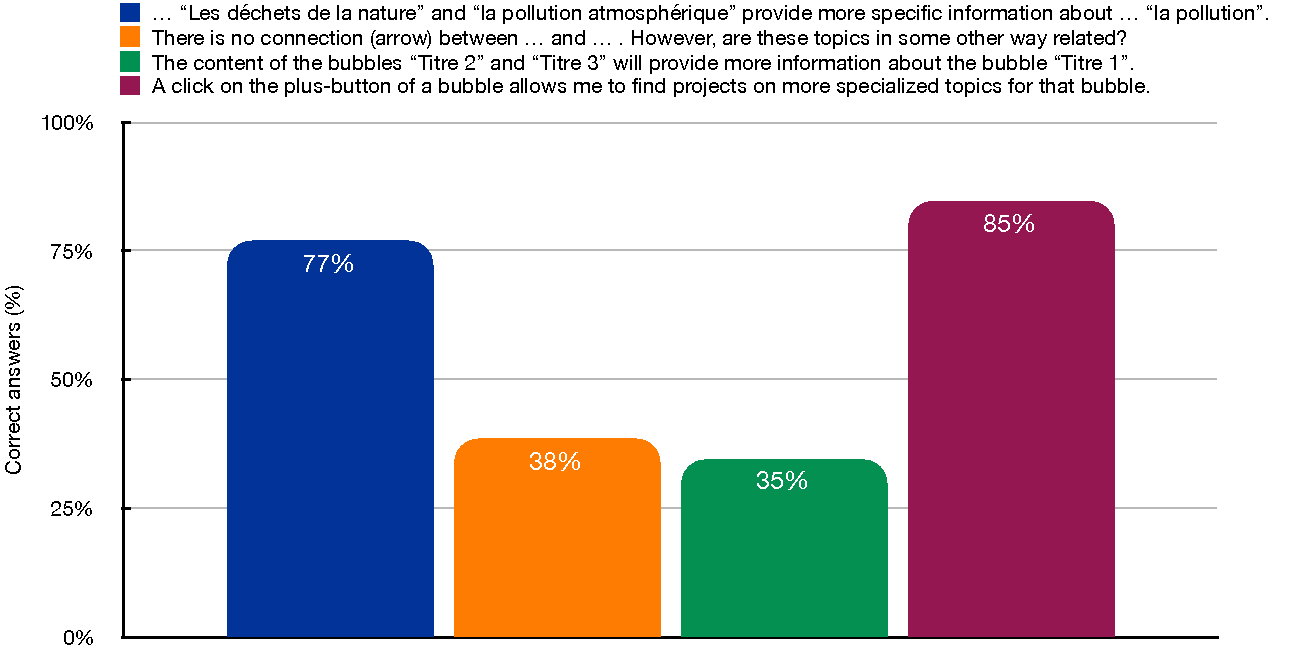
\includegraphics[width=\linewidth]{evaluation/part1-insight.pdf}}
	\caption{Results of insight questions.}
	\label{fig:evaluation-pdd-insight}
\end{figure}




%\begin{figure}[H]
%	\centering
%	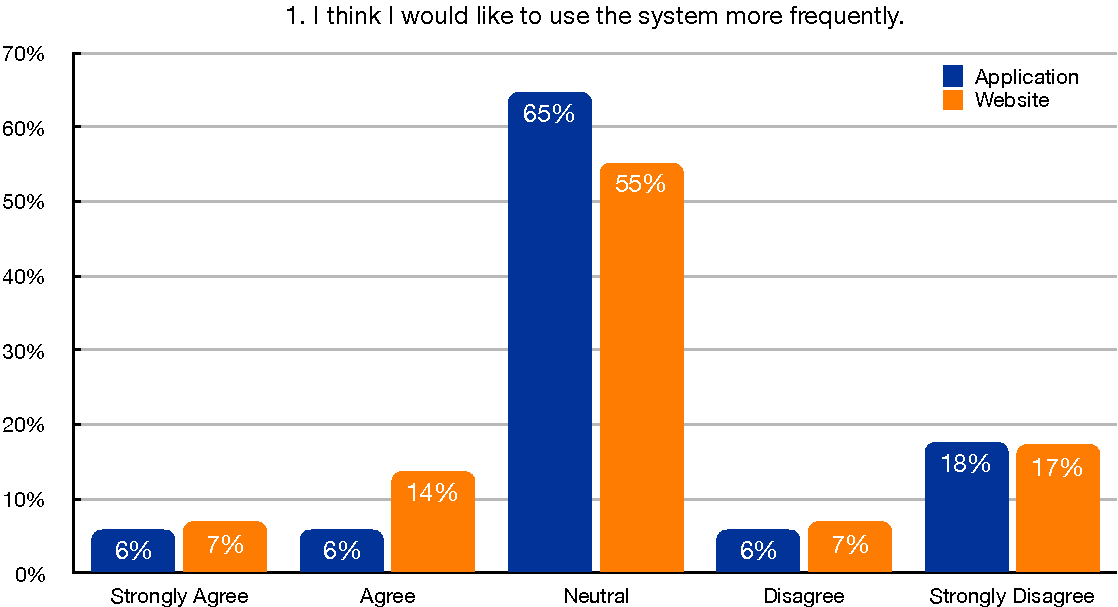
\includegraphics[width=.49\textwidth]{evaluation/usability-q1.pdf}
%	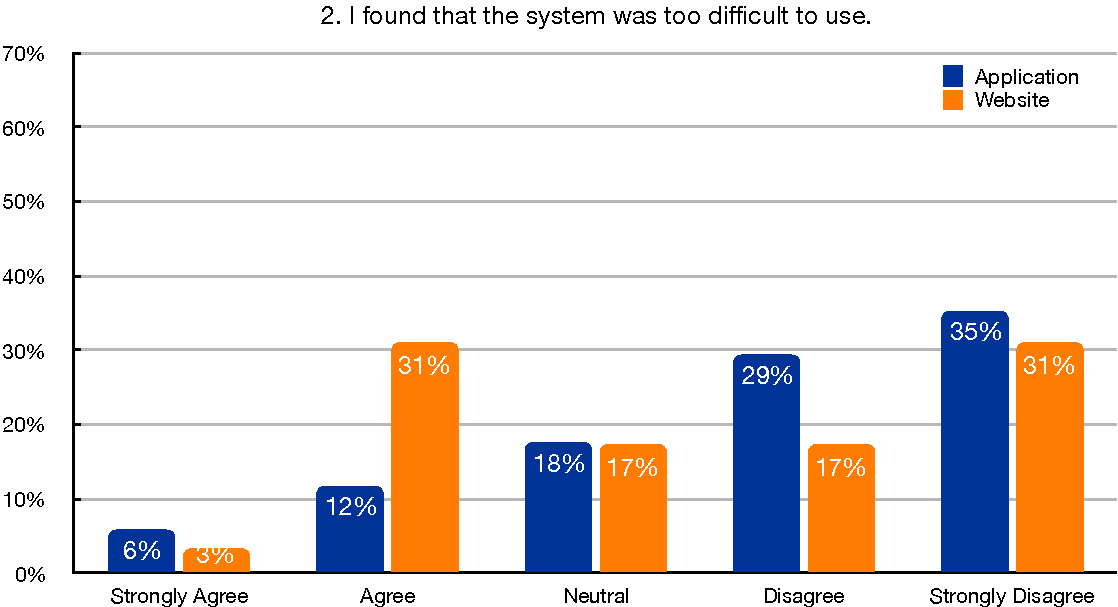
\includegraphics[width=.49\textwidth]{evaluation/usability-q2.pdf}
%	
%	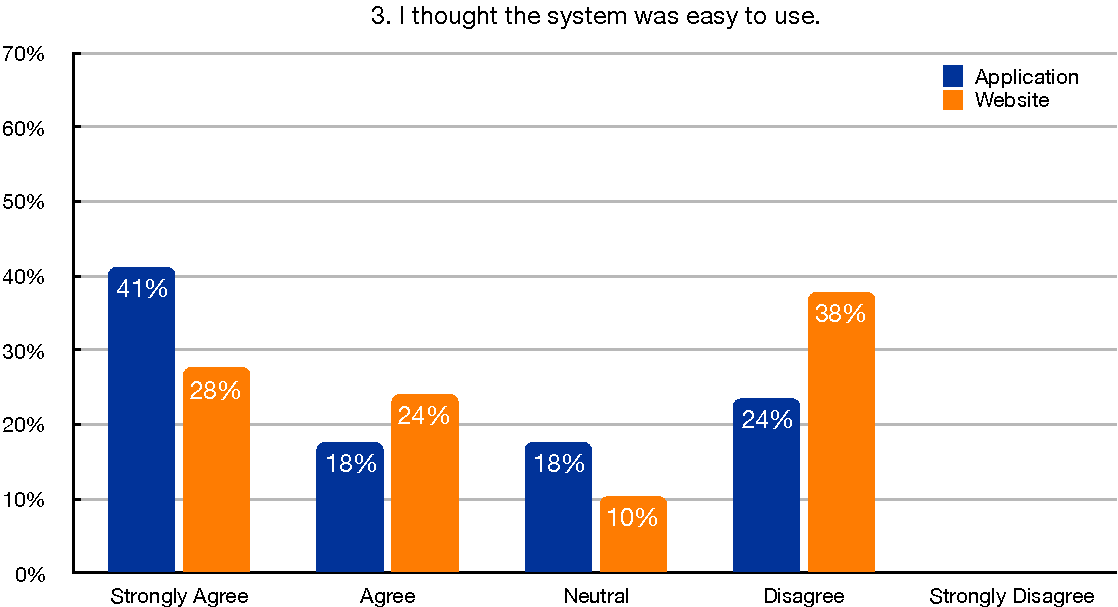
\includegraphics[width=.49\textwidth]{evaluation/usability-q3.pdf}
%	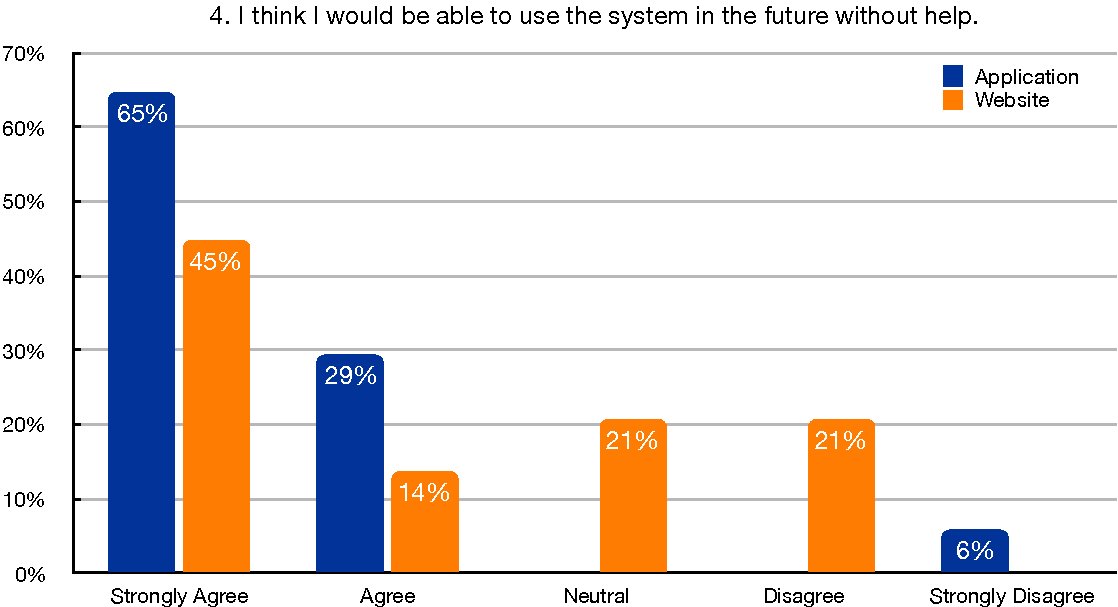
\includegraphics[width=.49\textwidth]{evaluation/usability-q4.pdf}
%	
%	\caption{test}
%\end{figure}

\subsubsection{Usability}
For the second part of the questionnaire, we expect the website is less usable than the visualization. Further, because we had more difficulties to search and find information on the website than in the application, we expect the user experience of the application will be better in comparison to the website. \\

\autoref{fig:evaluation-pdd-usability} shows eight graphs, each representing the results of one of the eight questions about usability of plateforme dd. When we look at the results of the first question, we can conclude that most of the participants whether they want to use the system more frequently or not.\\

In question two and three, we tested the simplicity of the website and the application. We see that the majority of the participants using the application (strongly) disagrees with the statement that the tool is too difficult to use. On the other hand, we see a peak of participants using the website who agree with the same statement. In the next statement, the opposite was asked. Here we can make similar conclusions. In case of the application, the majority answered this question with ``strongly agree'', while in case of the website an equal percentage answered ``disagree''. Hence, based on these two questions, we can conclude that the application was easier to use than the website.\\

Further, almost all participants using the application (all except 6\%) think they will be able to use the tool in the future without help. In case of the website, 40\% is still neutral or disagrees with this statement. The fifth question enforces this result even more: 80\% of the respondents using the application thinks their friends would be able to learn the system quickly, while in case of the website this is only 50\%.\\

We see that participants using the application agree quite often with the sixth question, ``I found it too much hassle to use the system'', while the majority using the website disagrees with this statement. This is probably because the application was a bit slower than expected on the used devices. As a consequence, the tool was not always responding immediately, which was sometimes confusing for the users.\\

Overall, based on the answers from this usability questionnaire, we can conclude that the application scores a bit better than the website. Hence, by creating the tool we succeeded in our intention to make the structure of the content more clear and more attractable than the website.


\begin{figure}[h]
	\centering
	\begin{subfigure}{.49\textwidth}
  		\centering
  		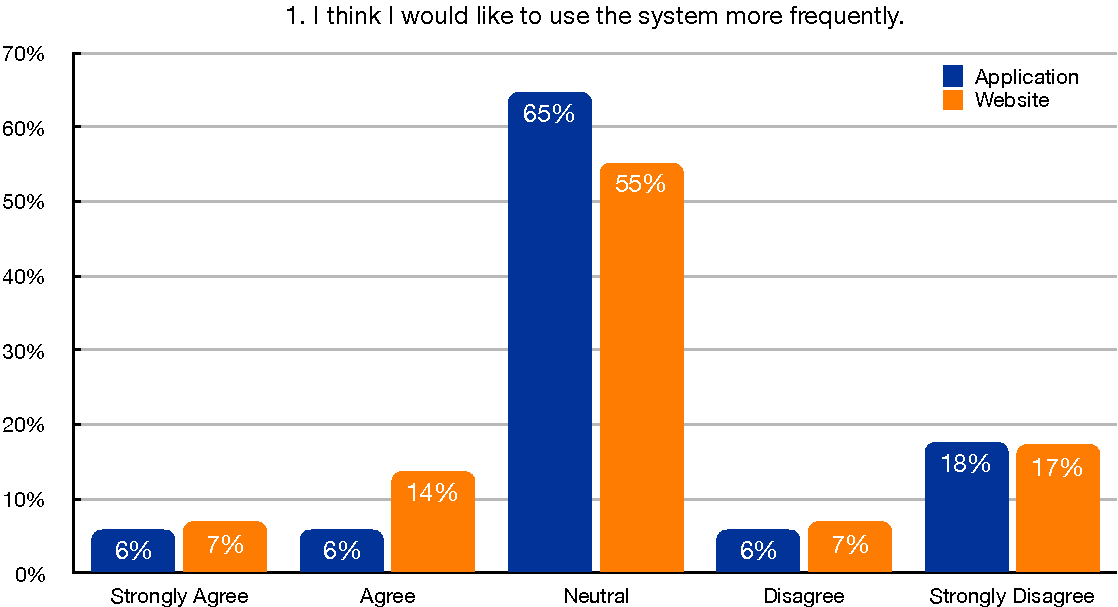
\includegraphics[width=\linewidth]{evaluation/usability-q1.pdf}
  		\caption{Results for question 1.}
  		%\label{fig:plusicon}
	\end{subfigure}%
	\begin{subfigure}{.49\textwidth}
  		\centering
  		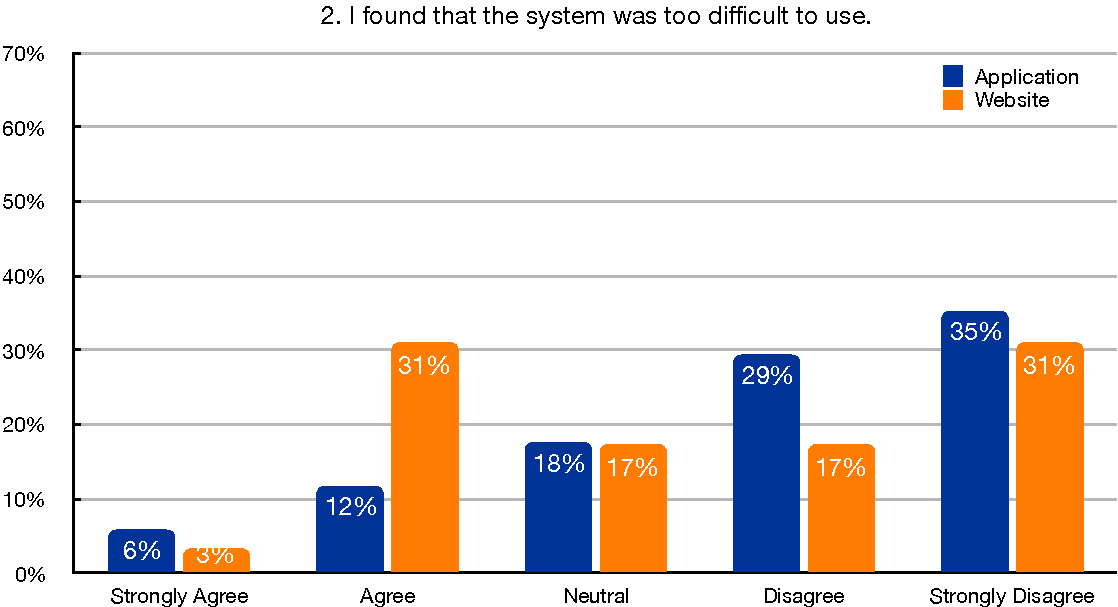
\includegraphics[width=\linewidth]{evaluation/usability-q2.pdf}
  		\caption{Results for question 2.}
  		%\label{fig:editicon}
	\end{subfigure}\par\bigskip
	
	\begin{subfigure}{.49\textwidth}
  		\centering
  		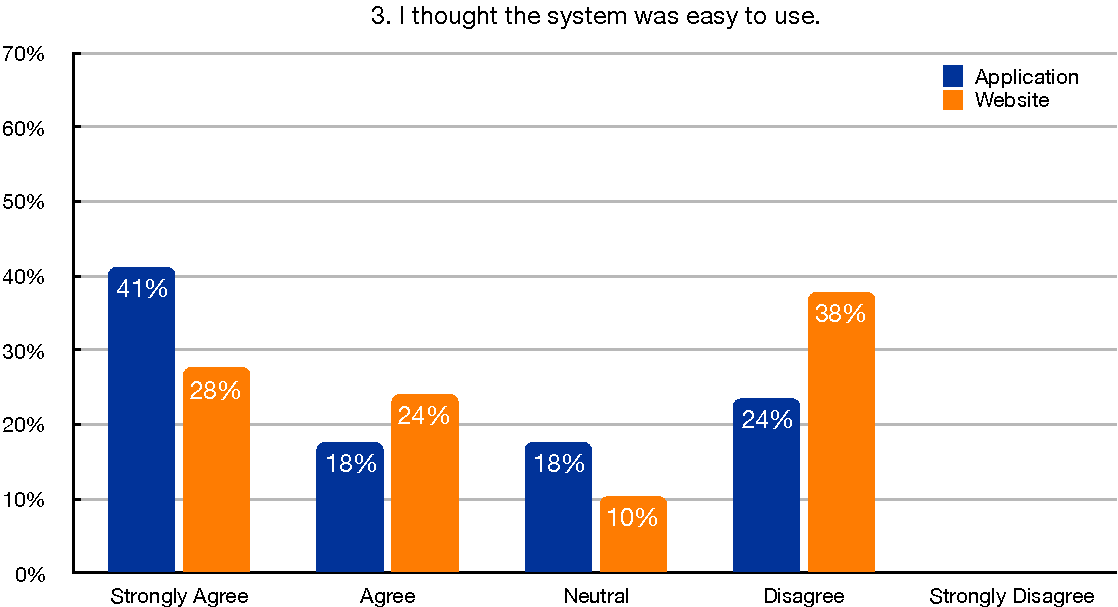
\includegraphics[width=\linewidth]{evaluation/usability-q3.pdf}
  		\caption{Results for question 3.}
  		%\label{fig:plusicon}
	\end{subfigure}%
	\begin{subfigure}{.49\textwidth}
  		\centering
  		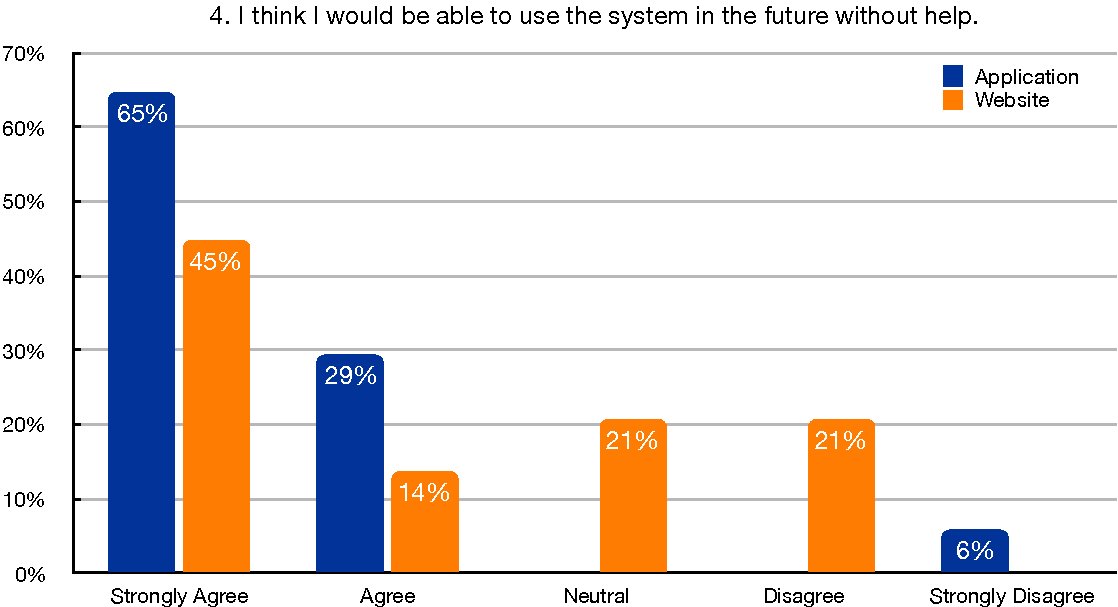
\includegraphics[width=\linewidth]{evaluation/usability-q4.pdf}
  		\caption{Results for question 4.}
  		%\label{fig:editicon}
	\end{subfigure}\par\bigskip
	
	\begin{subfigure}{.49\textwidth}
  		\centering
  		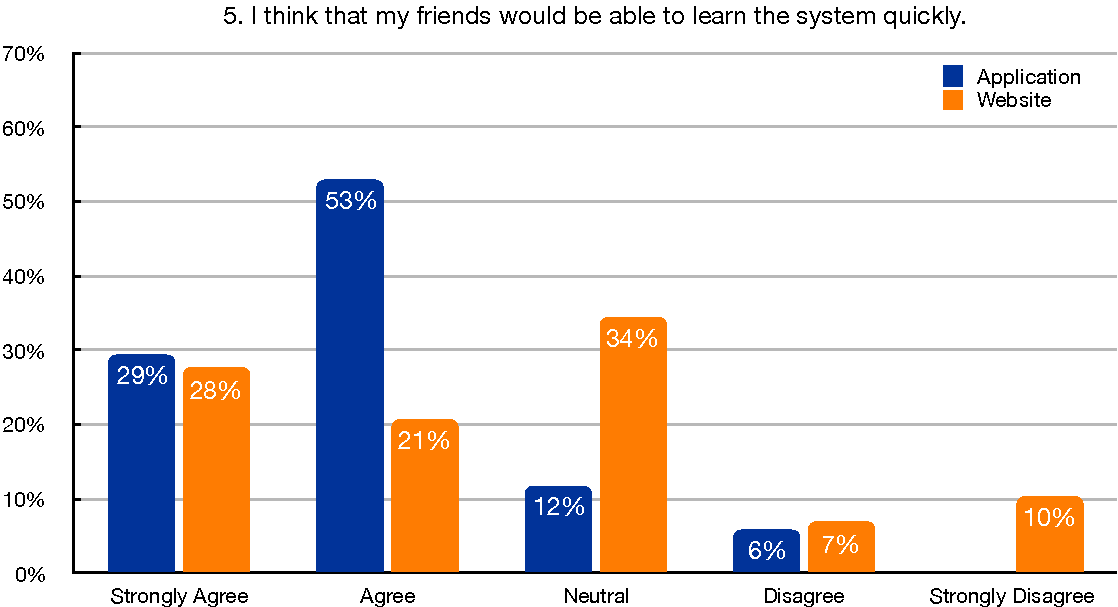
\includegraphics[width=\linewidth]{evaluation/usability-q5.pdf}
  		\caption{Results for question 5.}
  		%\label{fig:plusicon}
	\end{subfigure}%
	\begin{subfigure}{.49\textwidth}
  		\centering
  		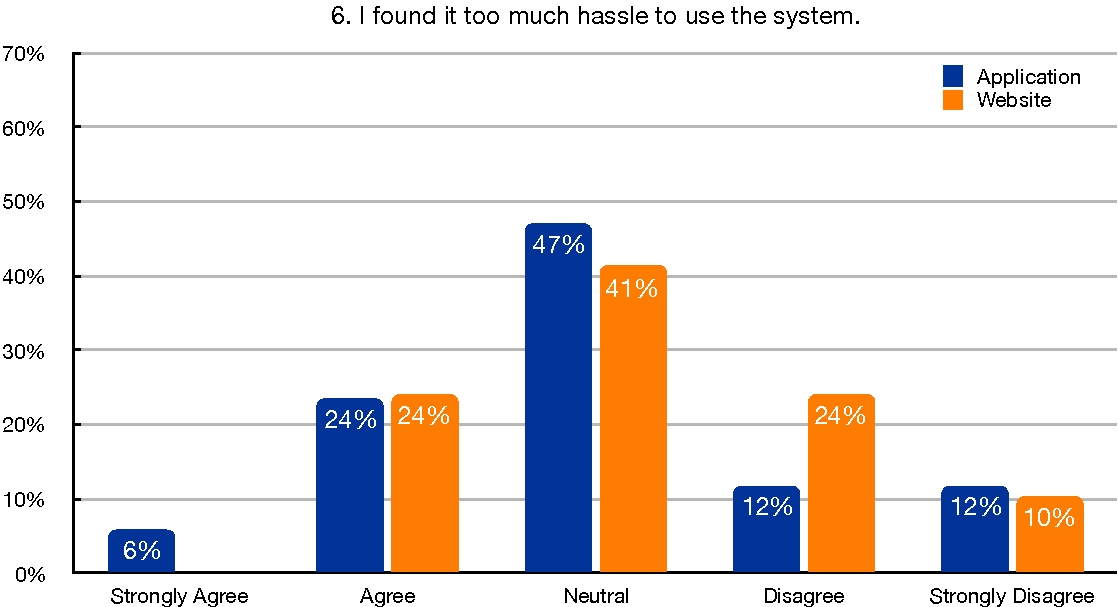
\includegraphics[width=\linewidth]{evaluation/usability-q6.pdf}
  		\caption{Results for question 6.}
  		%\label{fig:editicon}
	\end{subfigure}\par\bigskip
	
	\begin{subfigure}{.49\textwidth}
  		\centering
  		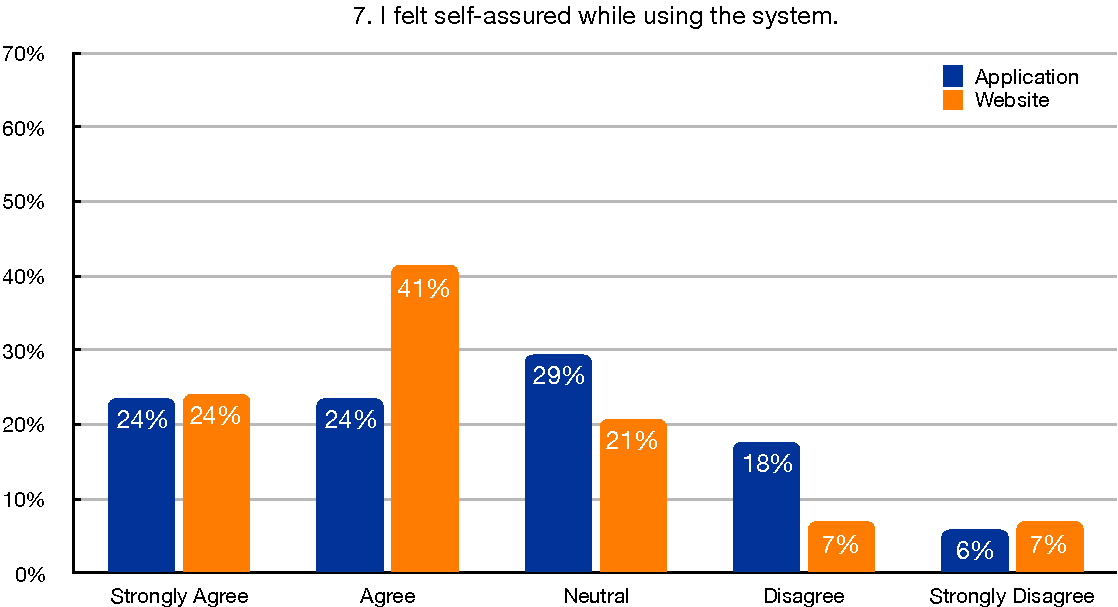
\includegraphics[width=\linewidth]{evaluation/usability-q7.pdf}
  		\caption{Results for question 7.}
  		%\label{fig:plusicon}
	\end{subfigure}%
	\begin{subfigure}{.49\textwidth}
  		\centering
  		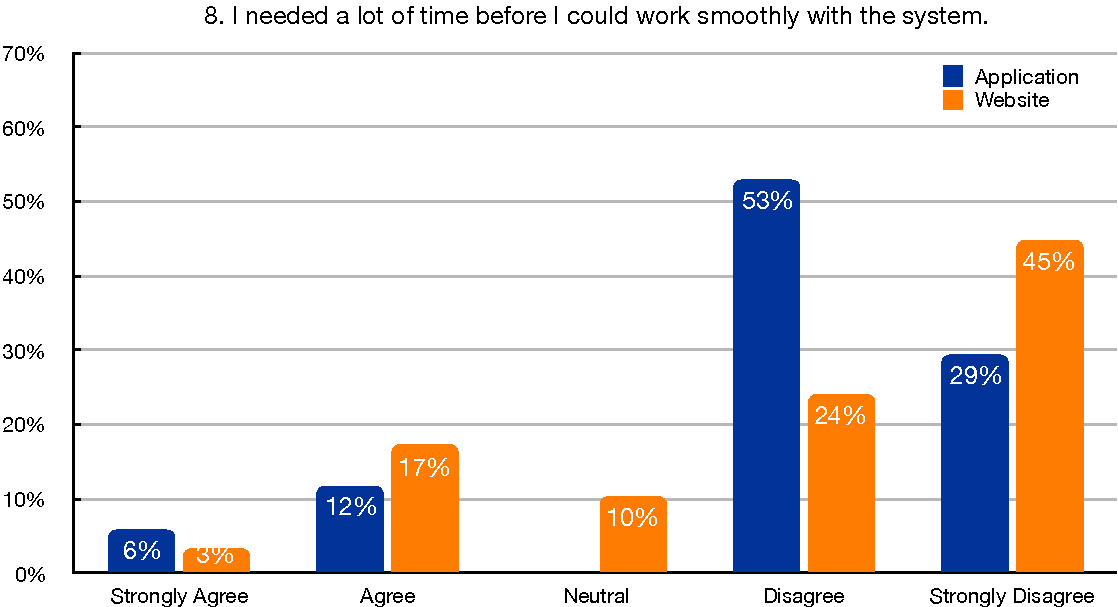
\includegraphics[width=\linewidth]{evaluation/usability-q8.pdf}
  		\caption{Results for question 8.}
  		%\label{fig:editicon}
	\end{subfigure}
	\caption{Usability Results Plateforme DD.}
	\label{fig:evaluation-pdd-usability}
\end{figure}

\subsubsection{User Experience}
To test the user experience, we used a questionnaire\footnote{\url{https://www.ueq-online.org/}} composed in such a way that inconsistencies can be easily detected. Together with the questionnaire, you can download an excel-file in which you have to insert all given answers. In the file, the answers are immediately analyzed and graphs are created for you.\\

The questionnaire consists of 26 terms at one side with their opposite at the other side. Between each to terms, the numbers one to seven can be found. The opposites are structured in such a way that the most negative of the two is not always number one or always number seven. Also, each couple of terms corresponds to one of six categories: attractiveness, perspicuity, efficiency, stimulation or novelty.\\

It is the task of the respondent to indicate the number which lies the closest to his opinion/feelings about the system he used. Afterwards we inserted all numbers in the excel-file, which converts the numbers from one to seven to a range between -3 and +3, where a -3 stands for the most negative answer and +3 for the most positive answer of the two. Then for each couple of opposites, the mean is taken for all converted answers. Hence, we get again a number between -3 and +3. Because it is very unlikely to have a mean lower than -2 and higher than 2, the graphs are created with a range between -2 and +2. This is also done because a mean of 1.5, which is already a quite good value, still seems to be less positive as it is on a scale from -3 to +3. The resulting graphs can be found in \autoref{fig:evaluation-pdd-ueq}.

\begin{figure}[h]
	\centering
	\begin{subfigure}{.49\textwidth}
  		\centering
  		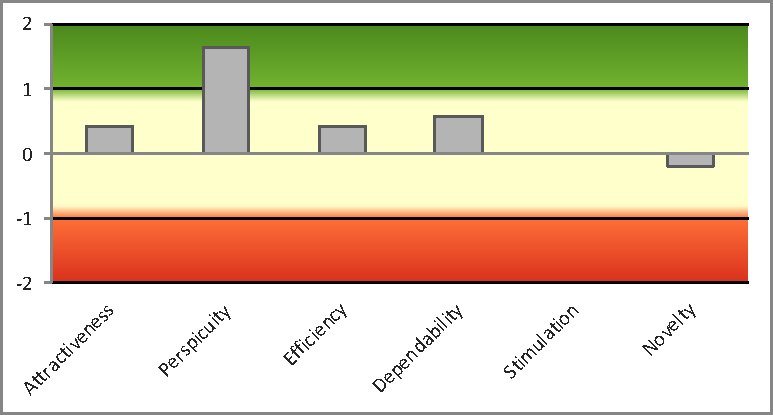
\includegraphics[width=\linewidth]{evaluation/evaluation-pdd-ueq-app.pdf}
  		\caption{Results User Experience Application}
  		%\label{fig:plusicon}
	\end{subfigure}%
	\begin{subfigure}{.49\textwidth}
  		\centering
  		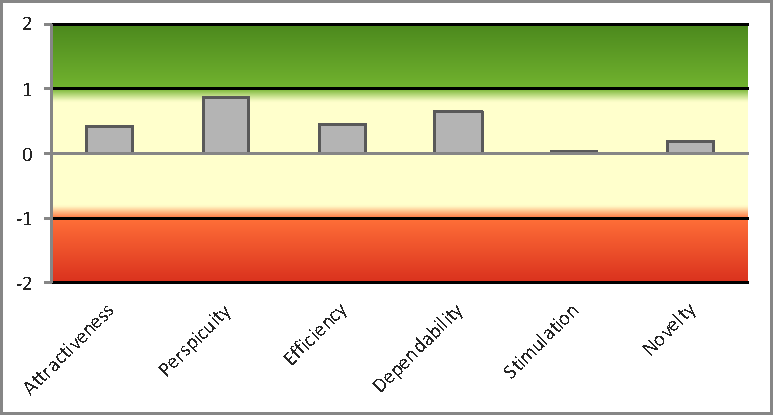
\includegraphics[width=\linewidth]{evaluation/evaluation-pdd-ueq-website.pdf}
  		\caption{Results User Experience Website}
  		%\label{fig:editicon}
	\end{subfigure}
	\caption{User Experience Results Plateforme DD.}
	\label{fig:evaluation-pdd-ueq}
\end{figure}

\color{black}



